%André Fernandes dos Santos
%LEI, nº49344

\documentclass{article}
\usepackage[portuguese,english]{babel}
\usepackage[utf8]{inputenc}
\usepackage[T1]{fontenc}
%\usepackage{a4wide}
\usepackage{txfonts}% use Arial && Times New Roman
\usepackage[pdftex]{color,graphicx}
\usepackage{fancyhdr}
\usepackage{fancyvrb}
\usepackage{longtable}
\usepackage{verbatim}
\usepackage{ae}
\usepackage{multicol}
\usepackage{graphicx}
\usepackage{hyperref}
\usepackage{url}
\usepackage{multicol}
\usepackage[defernumbers]{biblatex}
\usepackage{enumitem}

\addbibresource{aspubs}
\renewcommand\familydefault{\sfdefault}% usar font sem serifas
\renewcommand{\labelitemi}{$-$}

\author{André Fernandes dos Santos}
\title{Curriculum Vit\ae}
%\date{\today}
\date{June 28, 2012}

\begin{document}
\maketitle
%\thispagestyle{empty}

%\newpage
\section{Personal Information}
	\begin{description}
	\item [Name:] \large\textbf{\textsc{André Fernandes dos Santos}}
	\end{description}
\begin{multicols}{2}
	\begin{description}[style=multiline,leftmargin=5.5em]
	%\item [Nome:] \framebox{\textsc{André Fernandes dos Santos}}
	\item [Birthdate:] February 24, 1988
	\item [Address:] Pq. Resid. Fonte Seca,\\Lt8B 1$\,^{\circ}$E,\\4715-229 Braga\\PORTUGAL
	\item [Civil state:] Single
	\item [Phone:] +351 92 77 15 379
	\item [Email:] \href{mailto:andrefs@andrefs.pt}{andrefs@andrefs.pt}
	\end{description}
	\vfill

	\columnbreak
%	\begin{figure}[htbp]
%	\centering
%	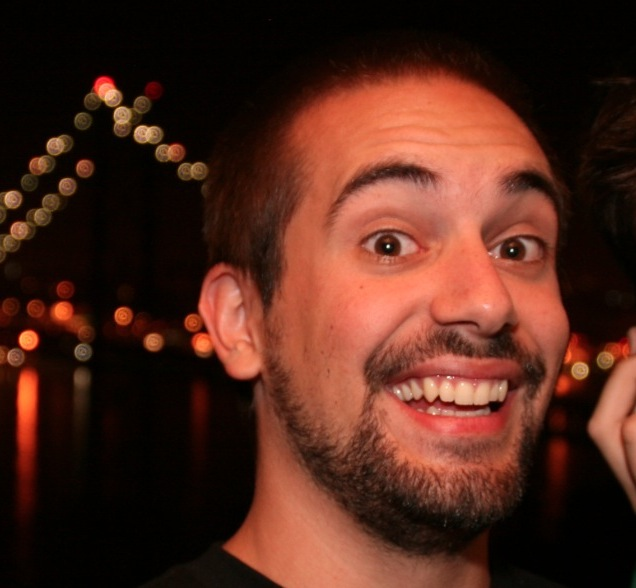
\includegraphics[width=.1\textwidth]{foto}
%	\end{figure}

	\begin{description}[style=multiline,leftmargin=5.5em]
		\small
		\item [Homepage:] 	\href{http://andrefs.pt}{andrefs.pt}
		\item [Twitter:] 	\href{http://twitter.com/about\_andrefs}{@about\_andrefs} 
		\item [GitHub:] 	\href{http://github.com/andrefs}{github.com/andrefs} 
		\item [LinkedIn:] 	\href{http://linkedin.com/in/andrefs}{linkedin.com/in/andrefs}
		\item [SlideShare:] \href{http://slideshare.net/andrefsantos}{slideshare.net/andrefsantos}
		\item [CPAN:] 		\href{http://search.cpan.org/~andrefs/}{search.cpan.org/~andrefs/}
	\end{description}
	\vspace*{\fill}
\end{multicols}


\section{Education}
%\begin{description}
\begin{tabular}{p{.18\textwidth}p{.8\textwidth}}
\textbf{2010-present} & MSc in Bioinformatics, University of Minho \newline
                       120 ECTS                                               \\
\textbf{2009-2011} & MSc in Natural Language Processing, University of Minho \newline
                     120 ECTS -- final grade 17/20                           \vspace{.2cm}\newline
                     Master thesis: ``Building a Corpora-Flow System''       \newline
                     {\small\textit{Development of a system to support automatic handling of corpora (cleaning, validation, format conversion), document alignment and calculation alignability metrics of several types of documents.}}\\
\textbf{2006-2009} & BSc in Software Engineering, University of Minho        \newline
                     180 ECTS, final grade 15/20                             \\
\end{tabular}

\section{Professional Experience}
\begin{description}
\item [Jul-Set 2009] Project Bigorna, Traineeship Sapo Summerbits 2009\\
\url{http://natura.di.uminho.pt/wiki/doku.php?id=ferramentas:bigorna}\\
Open source project which aims to develop natural language processing tools to help in general orthography migration challenges, motivated by the 1990 Portuguese Language Orthographic Agreement.
\item [Feb 2011 - present] Systems Administrator at GroupBuddies\\
\url{http://www.groupbuddies.com}\\
Startup company which develops web-based solutions for groups and organizations. Typical tasks include:
\begin{itemize}
	\item deployment and management of several Unix-based servers, with Apache and MySQL services
	\item managing Ruby on Rails applications on a production environment
	\item managing Git repositories
	\item development of helper scripts to automate and facilitate server management
	\end{itemize}
\item [Apr 2011 - present] Scholarship from project \textit{Per-Fide: Portuguese in parallel with six languages: Español, Russian, Français, Italiano, Deutsch, English}.\\
\url{http://per-fide.di.uminho.pt}\\
Project devoted to build large parallel corpora.

\end{description}


\section {Training}
\begin {description}
\item [Jul 2005] German Open Course, U. Junior, Faculty of Arts, University of Porto
\item [Set 2005] Physics Summer School, Faculty of Science, University of Porto
\item [Jun 2010] Catalyst 5.80 (\textit{Portuguese Perl Workshop 2010}, Porto)
\item [Jul 2010] Evolutionary Computing School, (UMinho, Guimarães)
%\item [Out 2010] Seminar ``Republic and Youth'', National Youth Council
\item [Nov 2010 - Mar 2011] IdeaLab -- Business Ideas Lab, TecMinho
\item [Jun 2011 - Jul 2011] Summer School on Conceptual Design and Development of Innovative Products 2011, Struer, Denmark (5 ECTS)
\end{description}


\section{Technical Skills}
\begin{description}
\item[-] Basic experience with PASCAL, C\#, PHP, JavaScript, UML, XML, HTML, SQL, Haskell;
\item[-] Experience with SQL and database management.
\item[-] Proficiency with C and Java;
\item[-] Proficiency with  Perl, including Moose, Catalyst, Dancer, DBIx::Class and other Modern::Perl concepts;
\item[-] Unix sys admin experience;
\item[-] Others: \LaTeX, bash, Subversion, Git, Apache and associated technologies.
\end{description}

\section{Other Activities}

\subsection{CeSIUM (UMinho's Software Engineering Student Center)}
\begin{description}
	\item [2008-2011] Member of CeSIUM 
	\item [2009/2010] Vice-President of CeSIUM 
	\item [2010/2011] Director of CAOS (Open Source Support Center)
\end{description}
\subsection{Programming Challenges}
\begin{description}
	\item [2007-2009] Inter-University Programming Marathon (IST'07, UC'08, ESTGA'09)
	\item [Nov 2008] ACM South Western European Regional Contests (Nuremberg, Germany)
	\item [Feb 2012] APPP Perl Code Sprint, 3$^\mathrm{rd}$ qualified
\end{description}
\subsection{Sports}
\begin{description}
	\item [1998-2000] Artistic gymnastics
	\item [2007-2008] Basketball
	\item [1999-2012] Judo, 4$\,^{\textrm{th}}$~Kyu
	\item [2010-2012] National Judo University Championship (Aveiro'10, Lisbon'11, Aveiro'12)
\end{description}


\nocite{*}
\printbibliography[nottype=misc,title=Publications]
\printbibliography[type=misc,title=Presentations]


\end{document}

